\section{Toolchain Analysis}
\label{sec-2-1}

All the methods mentioned above start with a complete definition of the toolchain. In OpenETCS, the development of the toolchain follows an \emph{agile} approach.
Hence, for each (major) release we have to deal with an incomplete tool
chain. In addition to the methods of the previous section,  we need a qualification
process that can adapt to the development speed, deal with an incomplete toolchain
and can re-use qualification information.

Moreover, as stated by Asplund et al., the toolchain provides some mechanism \textcolor{red}{[something is missing here]}
that has to be also ensured, reducing thereby the effort for each tool \cite{,asplund_towards_2012,asplund_qualifying_2012}. These
safety goals are related to the tool integration. In our context, most of  the tool
integration effort is made by integrating tools into a tool platform.
According to Asplund et al., the tool platform should ensure the following
safety-goals:
\begin{itemize}
\item Coherent time stamp information: common time stamps on development artifacts.
\item Notification: the user should be notified when artifacts changed.
\item Data integrity:  avoid use of obsolete artifacts, the data used reflects the
  current state.
\item Data mining: all data used by safety analysis should be available and be
  verifiable.
\end{itemize}

\section{OpenETCS Toolchain Qualification Process}
\label{sec-2-2}

The OpenETCS tool chain  will be defined by the set of its features and
a guideline describing how to correctly use it.
A SysML block diagram describes the tool chain architecture at a certain point in time as shown in
Figure \ref{fig:overview}. 
\begin{figure}[htbp]
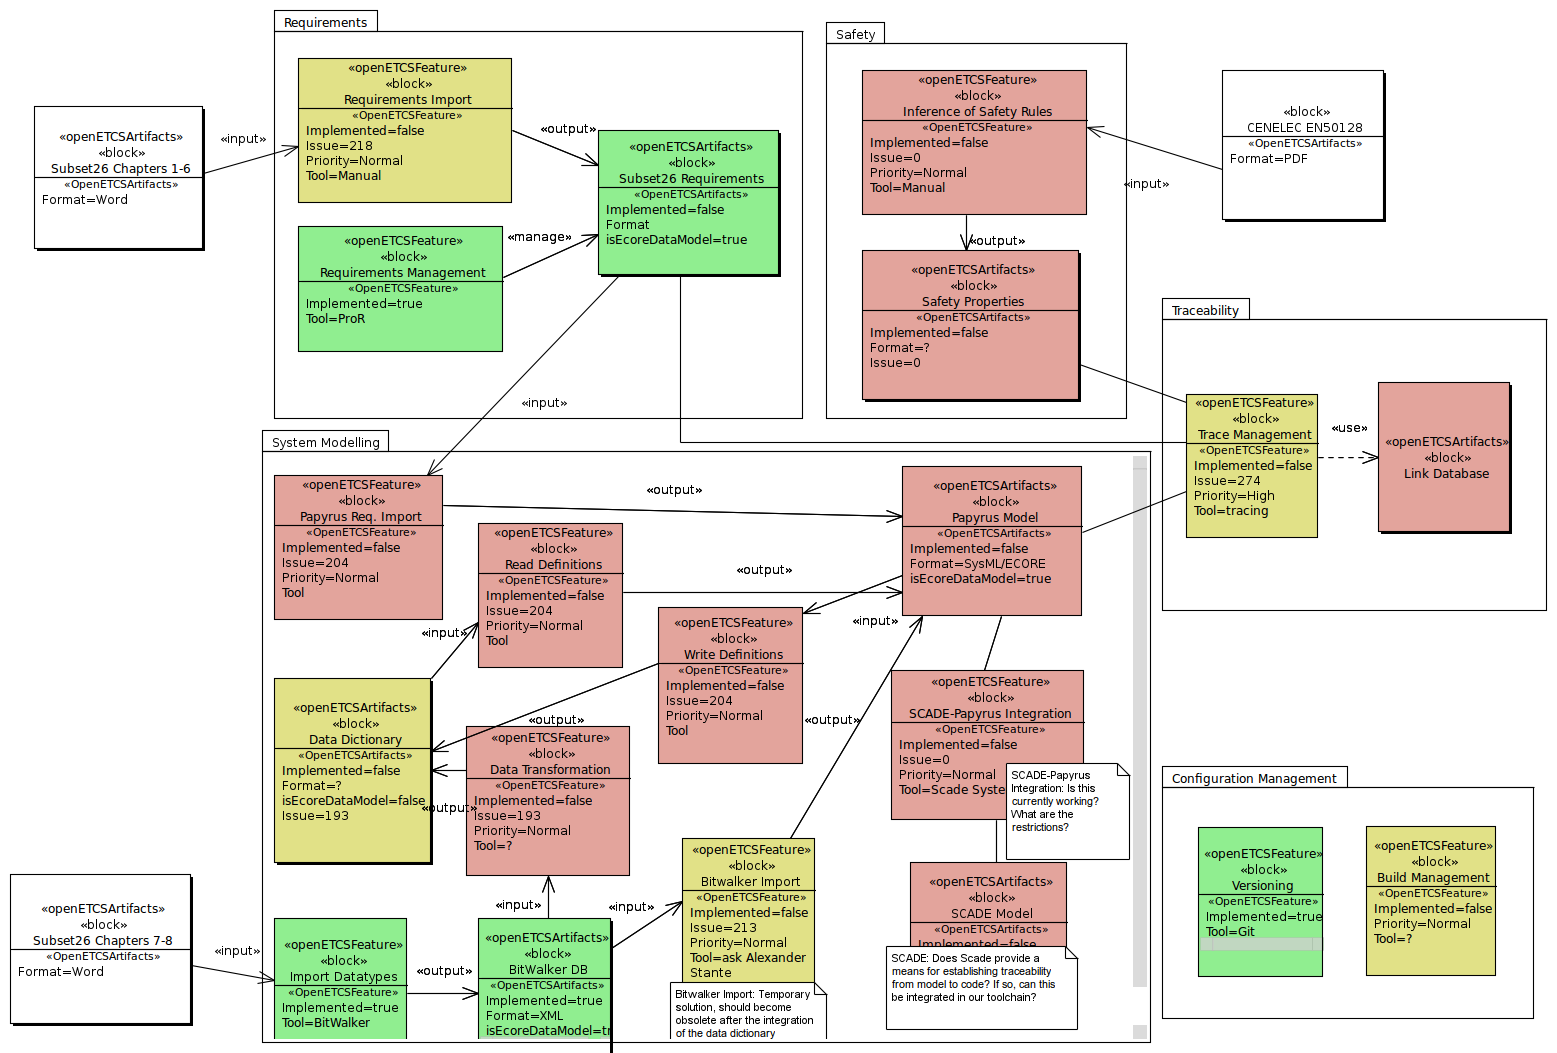
\includegraphics[width=\textwidth]{ToolChainmodel}
\caption{\label{fig:overview} Tool Chain overview (20.02.14) -- \\
  Green Block: Implemented \\
  Yellow Block: Work in Progress \\
  Red Block: Not started \\
  White Block: External Artifacts} 
\end{figure}

This block diagram is intended to grow according to new feature requests and the
needs of openETCS participants.  This diagram will be kept updated
as a reference of our tool chain. In any case, the complete information
regarding the feature availabilities  may be found in the Eclipse product
definition.

Each feature of the toolchain is a block with the profile ``openETCSFeature''
and  each artifact is block with the profile ``openETCSArtifact''.  Each
feature realizes at least one use case and may be implemented by one or more tools.
Note that in the tool platform features  may also be
implemented as plug-ins. The diagram also imposes a (partial) order
on the tasks. While some may be done in parallel, many tasks are dependent on others.
Currently, the diagram neither highlights the use of the tools, nor the order of actions
to be performed. This diagram should be completed by guidelines on
how to use the tool chain and/or an activity diagram.

To mitigate the qualification process, we will first consider more
than one feature at a time considering that errors from a tool A may
be detected by a Tool B in the next step of the tool chain process.
Furthermore, the toolchain is a collection
of features and not only tools. This differs from Asplund and al. in the sense that
some of the tool integration mechanisms that automate transformation of data, represent features
 and are thus not out of the scope of the qualification.

Due to our development process, a ``pre-qualification'' of tools should be made
when integrating a tool.

\marginpar{This high-level list should be detailed.}
\paragraph{Tool Integration Process for Qualification}

\begin{itemize}
\item Define name and version
\item Describe use cases
\item Provide justification of the tool within the tool chain
\item Provide input/output artifacts format (associated with the
  version)
\item Integrate the tool in the SysML model
\item Provide tool manual and other available documentation (associated with the version)
\item Link with an issue tracker
\end{itemize}

One possible implementation is to represent all these in formations
directly in the SysML model.

\marginpar{This high-level list should be detailed.  What I would expect: Which artefacts exist; How they are connected; When artefacts have to be re-validated (e.g. due to changes); What roles exist; who is responsible for what; etc.}
\paragraph{The Qualification Process}

\begin{enumerate}
\item Feature Analysis
  \begin{itemize}
  \item This step should assign a class to each feature based on the use cases.
  \item Define the potential errors
  \item Identify counter measure and/or error detection
  \item For T3 tools 2 alternatives:  certified compiler/generator or
    object code checker and/or exhaustive tester
  \end{itemize}
\item Tool platform  analysis 
  \begin{itemize}
  \item Provide evidence that the safety-goals mentioned in the
    previous sub-section are fulfilled\textcolor{red}{[The identification of safety goals is missing in step 1]}
  \end{itemize}
\item Toolchain Analysis
  \begin{itemize}
  \item Defines the work-flow
  \item Identify the ``hot spots'' of the toolchain
  \item Rearrange the toolchain if possible
  \item Find new measures when needed with combining tools (redundancy with orthogonal
    codes \ldots{})
  \end{itemize}
\item Toolchain qualification verification 
  \begin{itemize}
  \item Check consistency of tool version with  manuals and other
    provided feature information
  \item Generate table to  check if all possible errors has a
    detection or a correction mechanism
\item Generate the qualification report
  \end{itemize}

\end{enumerate}


\paragraph{An Example - Considerations for two openETCS Features}

\begin{longtable}{lp{0.7\textwidth}}
&\textbf{Bitwalker - Import of Data Types and Variables}\\
Input&Subset-026-7, Subset-026-8, MS Word Format\\
Output&Database (XML) representing data types, variables and messages\\
Tool Class&T3\\
          &The resulting definitions are direct input to the model and thus any fault may be propagated down to the code level\\
Safety Integrity Level&? \textcolor{red}{[Currently I do not have the EN 50128 standard available]}\\
Potential errors&The following list is not exhaustive and shall just give some ideas. The feature implementor has to provide more detail.
                                \begin{itemize}
                                  \item Variable / message / type not detected or missing in output\newline
                                       Mitigation: This error can possibly be detected avoided as the modelling process is manual. Required in- or output described in the
                                                   SRS can be added manually if missing.
                                  \item Variable or message have wrong type (*)\newline
                                       This is a very dangerous error, especially in the case of different precision integers or floats. The error may
                                       remain unnoticed and be propagated to the code leading to potentially fatal malfunctions. A mitigation is only possible by
                                       manual recheck (which would make an automatic conversion obsolete) of extensive/exhaustive testing or verification of the tool 
                                       implementing the feature. However the inconsistent nature of the input document (Word) could prevent this.
                                  \item Missing fields in record / message\newline
                                       Mitigation: Can be detected if the functionality of the field is described in the functional description.
                                  \item Wrong naming of variable / message / type (**)\newline
                                       Mitigation: Potentially dangerous if names of variables (of compatible type) are mixed up. The risk is the same as for wrong typing.
                                  \item ...
                                \end{itemize}
                               \\
Providing evidence&It will be necessary to provide evidence that critical errors such as (*) and (**) can be detected or are not present in the tool. 
                   Exhaustive verification will be difficult due to the unreliable structure of the input document. The result must be correct
                   also for ill-formed documents. A solution would be to let ERA acknowledge the converted XML database as a formal document. In this case the tool can be classified T1.

\end{longtable}



